\section{System Design}
\begin{frame}{Overview}
The model contain two main parts
\begin{itemize}
    \item Training Environment
    \item RL Model. 
\end{itemize}
\begin{center}
  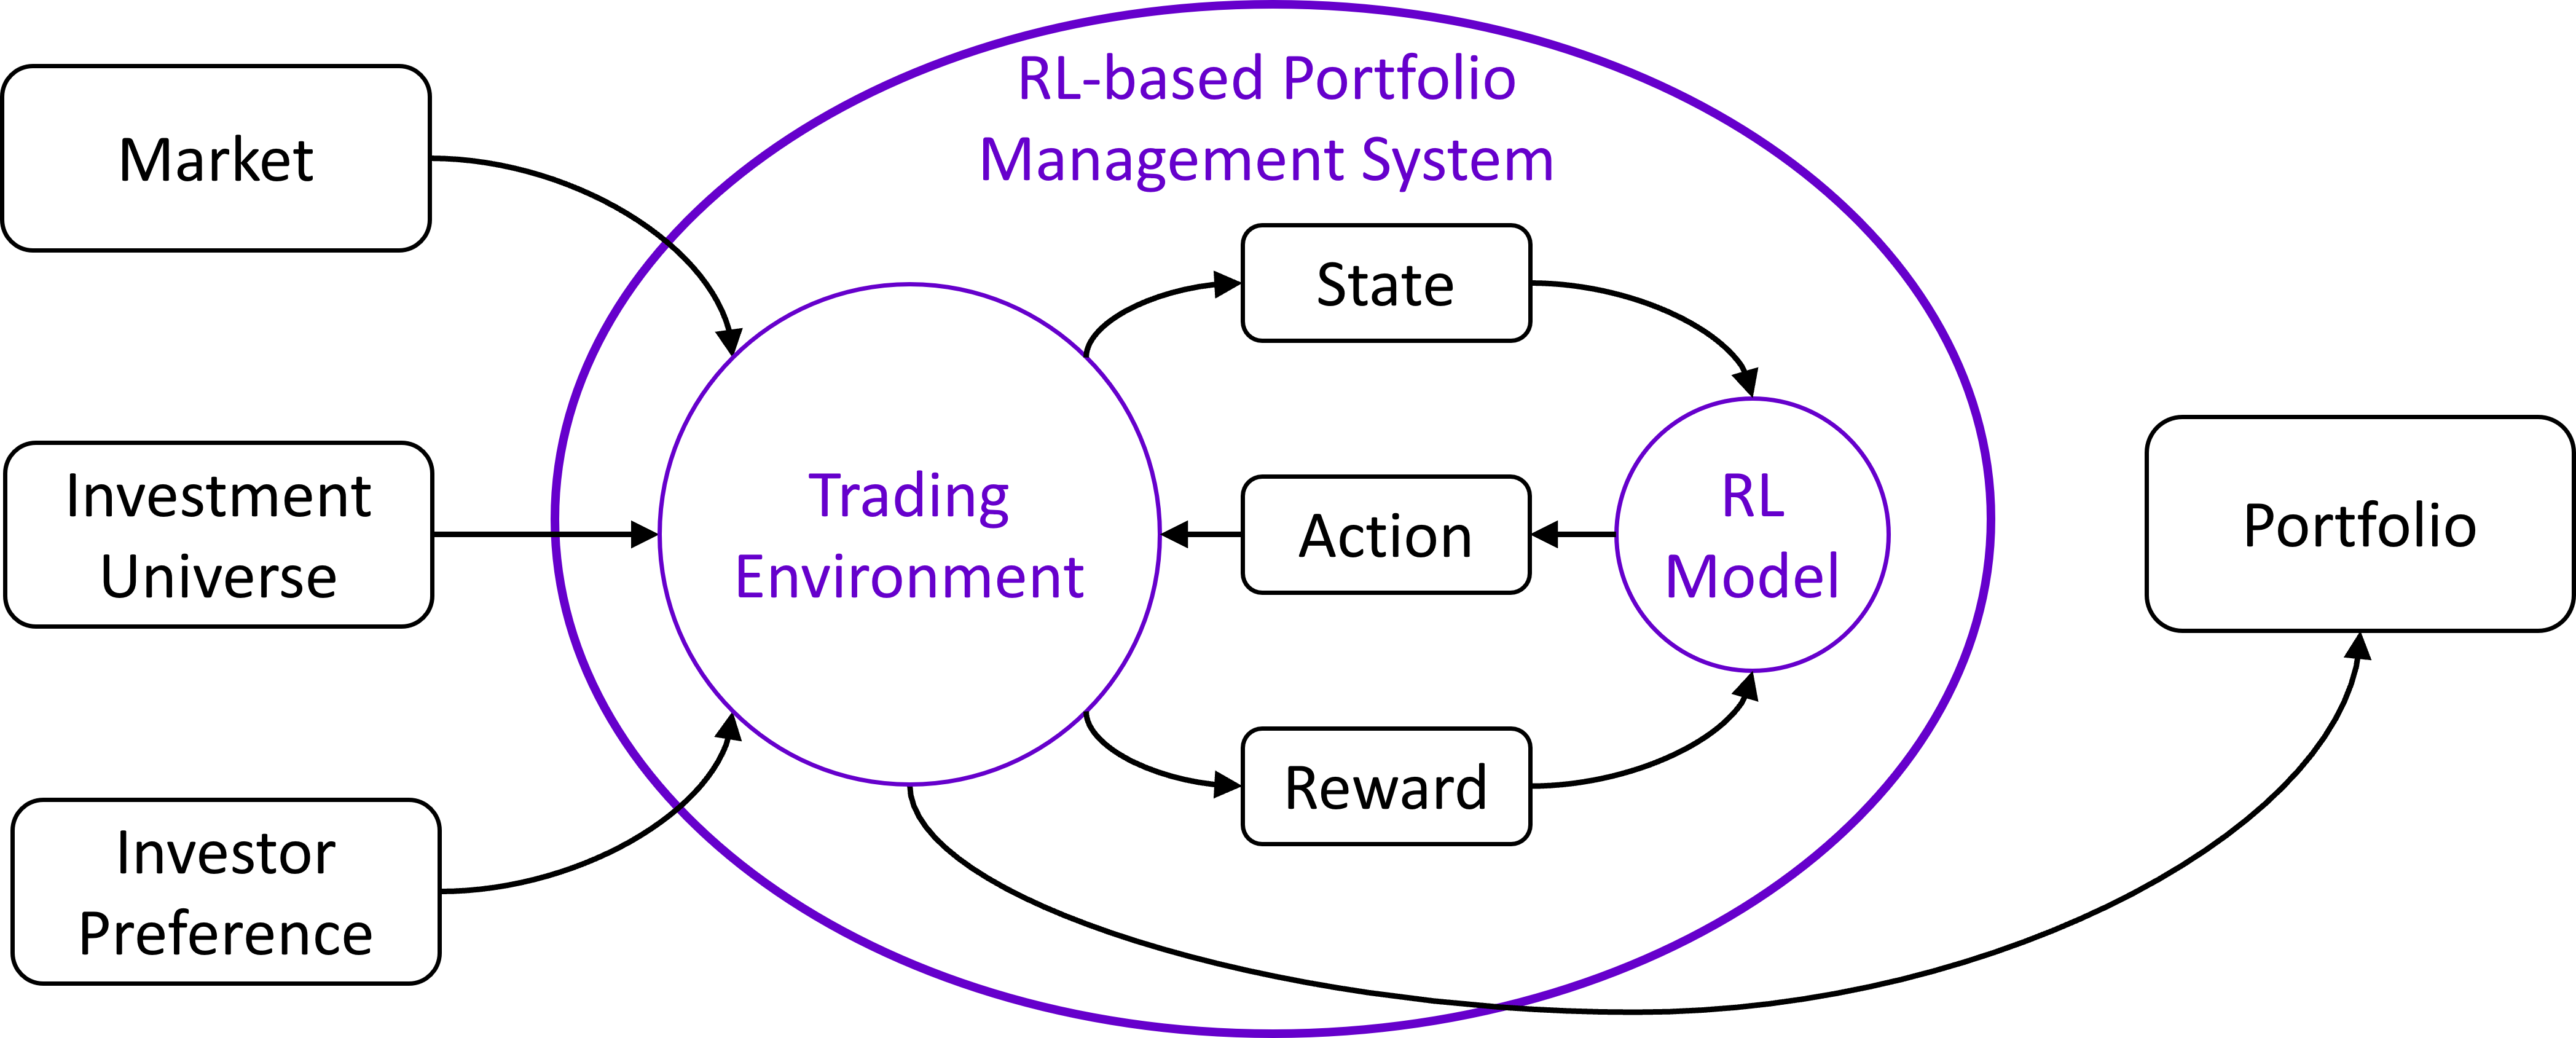
\includegraphics[width=10cm]{images/context_diagram.png}  
\end{center}
\end{frame}




\begin{frame}{Market Features}
\begin{block}{Structured information}
\begin{itemize}
    \item Interest rates
    \item Commodity prices
    \item Currency exchange indexes
    \item Other Indexes
\end{itemize}
\end{block}
\begin{block}{Stationary data}
   Use directly as features
\end{block}
\begin{block}{Non-stationary data}
    Use statistics measures among 5, 20, and 60 days as features, including standard deviation, skewness, and kurtosis.
\end{block}
\end{frame}

\begin{frame}{Market Features}
\footnotesize
\begin{tabular}{|| c| c | c||}
\hline
Description & Categories & Stationary \\ \hline \hline
5-Year Treasury Constant Maturity Rate & Interest Rates  & Yes \\ \hline
10-Year Treasury Constant Maturity Rate & Interest Rates & Yes \\ \hline
30-Year Treasury Constant Maturity Rate & Interest Rates & Yes \\ \hline
5-Year Breakeven Inflation Rate & Interest Rates & Yes \\ \hline
10-Year Breakeven Inflation Rate & Interest Rates & Yes \\ \hline
Crude Oil Prices: Brent - Europe &  Commodities & No \\ \hline
Gold Prices &  Commodities & No \\ \hline
CBOE Volatility Index (VIX) &  Indexes & No \\ \hline
US Dollar Index (USDX) &  Currencies & No \\ \hline
\end{tabular}
\end{frame}



\newcommand\mynum[1]{{\renewcommand{\insertenumlabel}{#1}%
      \usebeamertemplate{enumerate item}}}

\begin{frame}{Investment Universe}
\begin{block}{Goal}
Choose 10 investments with low covariances between each other; hence their combinations can yield better profits from the same risk level
\end{block}
\begin{block}{Selection Process}
    \begin{enumerate}
    \item Starts from the top 100 ETFs by Asset Under Management (AUM)
    \item Remove ones with trading records of less than 14 years.
    \item \label{itm:remove_items} Obtain the top two most correlated ETFs and remove the one with lower AUM
    \item Repeat \mynum{\ref{itm:remove_items}} iteratively until 10 ETFs are left
    \end{enumerate}
\end{block}
\end{frame}

\begin{frame}{Selection of ETFs}
    \begin{tabular}{|| c | c ||}
    \hline
    Symbol & Name  \\ \hline \hline
    SPY&SPDR S\&P 500 ETF \\ \hline
    AGG&iShares Core U.S. Aggregate Bond ETF \\ \hline
    BND&Vanguard Total Bond Market ETF \\ \hline
    GLD&SPDR Gold Trust \\ \hline
    LQD&iShares iBoxx \$ Investment Grade Corporate Bond ETF \\ \hline
    BSV&Vanguard Short-Term Bond ETF \\ \hline
    MBB&iShares MBS Bond ETF \\ \hline
    IGSB&iShares Short-Term Corporate Bond ETF \\ \hline
    SHY&iShares 1-3 Year Treasury Bond ETF \\ \hline
    SHV&iShares Short Treasury Bond ETF \\ \hline
    \end{tabular}
\end{frame}



\begin{frame}{Investor Preference}
For investor preference, we focus on risk.
\begin{block}{Acquire risk aversion}
Professional personnel or organization will acquire risk aversion from investors by survey or other techniques and interprets the inputs into comparable indicators, e.g., MDD, between investors.
\\
\alert{This part is not in the scope of our thesis}
\end{block}
\begin{block}{Risk Indicator}
We use MDD as the risk indicator to evaluate our system. However, optimizing any ratio using MDD directly has many challenges. Some researches indicate MDDs are outliers or imply optimizing MDD is troublesome. 
\\
\alert{We will not limit ourselves to use MDD while optimizing the model and consider other alternatives.}
\end{block}
\end{frame}






